\documentclass[12pt,a4paper]{article}

% ── Packages ──────────────────────────────────────────────────
\usepackage{amsmath,amssymb,amsthm}
\usepackage{geometry}
\geometry{left=2.5cm,right=2.5cm,top=2.5cm,bottom=2.5cm}
\setlength{\headheight}{14pt}
\usepackage{graphicx}
\usepackage{booktabs}
\usepackage{array}
\usepackage{hyperref}
\usepackage{fancyhdr}
\usepackage{enumitem}
\usepackage{caption}
\usepackage{float}
\usepackage{algorithm}
\usepackage{algpseudocode}
\usepackage{xcolor}

\usepackage{parskip}
\usepackage{setspace}
\usepackage{tcolorbox}
\tcbuselibrary{theorems, breakable, skins}
\usepackage{mdframed}
\usepackage{tikz}
\usepackage{pgfplots}
\pgfplotsset{compat=1.18}

% Cấu hình Tiếng Việt chuẩn cho XeLaTeX / LuaLaTeX
\usepackage{fontspec}
\usepackage[vietnamese]{babel}
\setmainfont{Times New Roman} % Hoặc Arial, Calibri tùy sở thích (Yêu cầu biên dịch bằng XeLaTeX)

% ── Colors ───────────────────────────────────────────────────
\definecolor{defblue}{RGB}{30,90,160}
\definecolor{defbluebg}{RGB}{235,243,255}
\definecolor{thmgreen}{RGB}{20,120,60}
\definecolor{thmbg}{RGB}{230,248,238}
\definecolor{noteorange}{RGB}{200,100,20}
\definecolor{notebg}{RGB}{255,243,220}
\definecolor{remarkgray}{RGB}{80,80,80}
\definecolor{remarkbg}{RGB}{245,245,245}

% ── tcolorbox styles ─────────────────────────────────────────

% Definition box (blue) — matches the PDF style
\newtcolorbox{definitionbox}[1]{
  enhanced,
  breakable,
  colback=defbluebg,
  colframe=defblue,
  fonttitle=\bfseries\small,
  title={Định nghĩa: #1},
  attach boxed title to top left={yshift=-2mm, xshift=4mm},
  boxed title style={colback=defblue, colframe=defblue, rounded corners},
  arc=3pt,
  left=6pt, right=6pt, top=8pt, bottom=6pt,
  before skip=10pt, after skip=10pt,
}

% Theorem box (green)
\newtcolorbox{theorembox}[1]{
  enhanced,
  breakable,
  colback=thmbg,
  colframe=thmgreen,
  fonttitle=\bfseries\small,
  title={Định lý: #1},
  attach boxed title to top left={yshift=-2mm, xshift=4mm},
  boxed title style={colback=thmgreen, colframe=thmgreen, rounded corners},
  arc=3pt,
  left=6pt, right=6pt, top=8pt, bottom=6pt,
  before skip=10pt, after skip=10pt,
}

% Note / Ghi chú box (orange)
\newtcolorbox{notebox}{
  enhanced,
  breakable,
  colback=notebg,
  colframe=noteorange,
  fonttitle=\bfseries\small,
  title={Ghi chú},
  attach boxed title to top left={yshift=-2mm, xshift=4mm},
  boxed title style={colback=noteorange, colframe=noteorange, rounded corners},
  arc=3pt,
  left=6pt, right=6pt, top=8pt, bottom=6pt,
  before skip=10pt, after skip=10pt,
}

% Remark box (gray)
\newtcolorbox{remarkbox}[1]{
  enhanced,
  breakable,
  colback=remarkbg,
  colframe=remarkgray,
  fonttitle=\bfseries\small,
  title={#1},
  attach boxed title to top left={yshift=-2mm, xshift=4mm},
  boxed title style={colback=remarkgray, colframe=remarkgray, rounded corners},
  arc=3pt,
  left=6pt, right=6pt, top=8pt, bottom=6pt,
  before skip=10pt, after skip=10pt,
}

% ── Header / Footer ──────────────────────────────────────────
\pagestyle{fancy}
\fancyhf{}
\fancyhead[L]{\small\textbf{Ho Chi Minh University of Science -- VNUHCM}}
\fancyhead[R]{\small Faculty of Information Technology}
\fancyfoot[L]{\small Applied Mathematics in Statistics}
\fancyfoot[R]{\small Page \thepage}
\renewcommand{\headrulewidth}{0.4pt}
\renewcommand{\footrulewidth}{0.4pt}

\setlength{\parskip}{6pt}
\setlength{\parindent}{0pt}

\begin{document}

% ══════════════════════════════════════════════════════════════
% TITLE PAGE
% ══════════════════════════════════════════════════════════════
\begin{titlepage}
\centering
\textbf{\large VIETNAM NATIONAL UNIVERSITY HO CHI MINH CITY}\\
\textbf{\large HO CHI MINH CITY UNIVERSITY OF SCIENCE}\\
\textbf{\large FACULTY OF INFORMATION TECHNOLOGY}\\[0.5cm]
\textbf{\large DEPARTMENT OF COMPUTER SCIENCE}\\[2cm]

\rule{\textwidth}{1pt}\\[0.5cm]
\textbf{\LARGE REPORT}\\[0.3cm]
\textbf{\Large Elastic Net và Polynomial Regression}\\[0.2cm]
\textbf{\Large cho Bài Toán Dự Đoán Chi Phí Du Lịch Tanzania}\\[0.3cm]
\rule{\textwidth}{1pt}\\[2cm]

\begin{tabular}{l l l}
\textbf{Lecturer:} & ThS. Võ Nam Thục Đoan & \\
                   & ThS. Lê Nhựt Nam & \\[0.3cm]
\textbf{Leader:}   & Khang Phuc Nguyen & 24120068 \\
\textbf{Members:}  & Nghia Trong Hoang & 24120103 \\
                   & Nhat Hoang Mai    & 24120109 \\
                   & Nhat Hoang Nguyen & 24120110 \\
                   & Long Nhat Phung Vo & 24120088 \\
\end{tabular}\\[3cm]

Ho Chi Minh City, 5/2026
\end{titlepage}

% ══════════════════════════════════════════════════════════════
% TABLE OF CONTENTS
% ══════════════════════════════════════════════════════════════
\tableofcontents
\newpage

% ══════════════════════════════════════════════════════════════
% 1. CƠ SỞ LÝ THUYẾT
% ══════════════════════════════════════════════════════════════
\section{Cơ Sở Lý Thuyết}

Báo cáo này trình bày hai phương pháp học máy quan trọng: \textbf{Elastic Net Regression} và \textbf{Polynomial Regression}, được áp dụng vào bài toán dự đoán chi phí du lịch tại Tanzania. Trong khi báo cáo trước đã khảo sát OLS, Ridge, và Lasso trên không gian đặc trưng One-Hot (186 features), báo cáo này mở rộng theo hai hướng: (1) kết hợp ưu điểm của cả Lasso và Ridge thông qua Elastic Net, và (2) khai thác các mối quan hệ phi tuyến giữa các biến số thông qua Polynomial Features.

Việc hiểu rõ nền tảng lý thuyết là bước không thể thiếu trước khi triển khai thực nghiệm, vì mỗi phương pháp đều có những giả thiết và điều kiện áp dụng riêng. Phần này sẽ trình bày chi tiết công thức toán học, ý nghĩa hình học, và mối liên hệ giữa các phương pháp.

\subsection{Elastic Net Regression}

Elastic Net là một trong những phương pháp chính quy hóa tinh vi nhất trong họ các mô hình hồi quy tuyến tính. Được đề xuất bởi Zou và Hastie năm 2005 \cite{zou2005}, Elastic Net ra đời để giải quyết một hạn chế cụ thể của Lasso: khi các biến có tương quan cao với nhau, Lasso có xu hướng chọn ngẫu nhiên một trong số chúng và loại bỏ phần còn lại, dẫn đến mô hình không ổn định và khó diễn giải. Elastic Net khắc phục điều này bằng cách kết hợp cả hai cơ chế phạt $L_1$ và $L_2$ trong một bài toán tối ưu hóa thống nhất.

Để hiểu rõ hơn vị trí của Elastic Net trong không gian các phương pháp chính quy hóa, ta có thể hình dung nó như một cầu nối giữa Ridge (chỉ dùng $L_2$, không thực hiện feature selection) và Lasso (chỉ dùng $L_1$, thực hiện feature selection mạnh nhưng không ổn định với correlated features). Elastic Net cho phép kiểm soát linh hoạt mức độ nghiêng về phía nào thông qua siêu tham số $\rho$.

\begin{definitionbox}{Elastic Net Regression}
Elastic Net là phương pháp hồi quy chính quy hóa kết hợp penalty $L_1$ (Lasso) và $L_2$ (Ridge), được đề xuất bởi Zou và Hastie (2005). Bài toán tối ưu có dạng:
\begin{equation}
\hat{\boldsymbol{\beta}}_{\text{EN}} = \arg\min_{\boldsymbol{\beta}} \left\{ \frac{1}{2n} \|\mathbf{y} - \mathbf{X}\boldsymbol{\beta}\|_2^2 + \alpha \left[ \frac{1-\rho}{2}\|\boldsymbol{\beta}\|_2^2 + \rho\|\boldsymbol{\beta}\|_1 \right] \right\}
\end{equation}
trong đó $\alpha \geq 0$ là tham số chính quy hóa tổng thể và $\rho \in [0,1]$ (\texttt{l1\_ratio}) kiểm soát tỷ lệ giữa $L_1$ và $L_2$.
\end{definitionbox}

\textbf{Ý nghĩa của từng thành phần trong bài toán tối ưu:}

Thành phần thứ nhất $\frac{1}{2n}\|\mathbf{y} - \mathbf{X}\boldsymbol{\beta}\|_2^2$ là hàm mất mát bình phương trung bình (MSE), đo lường mức độ sai lệch giữa dự đoán và giá trị thực. Thành phần thứ hai $\alpha\left[\frac{1-\rho}{2}\|\boldsymbol{\beta}\|_2^2 + \rho\|\boldsymbol{\beta}\|_1\right]$ là hàm phạt kết hợp, trong đó $\alpha$ kiểm soát tổng mức độ phạt và $\rho$ phân bổ mức phạt giữa $L_1$ và $L_2$.

\textbf{Các trường hợp đặc biệt:}
\begin{itemize}[leftmargin=1.5em]
    \item $\rho = 0$: Elastic Net $\equiv$ Ridge Regression (chỉ penalty $L_2$). Các hệ số được co lại nhưng không bao giờ bằng 0.
    \item $\rho = 1$: Elastic Net $\equiv$ Lasso Regression (chỉ penalty $L_1$). Cho phép đặt một số hệ số chính xác bằng 0.
    \item $0 < \rho < 1$: Kết hợp cả hai, vừa co hệ số (shrinkage) vừa loại biến (sparsity).
\end{itemize}

\begin{remarkbox}{So sánh Elastic Net với Lasso thuần}
Khi các biến có tương quan cao, Lasso có xu hướng chọn ngẫu nhiên một biến và loại bỏ các biến còn lại, dẫn đến tính không ổn định của mô hình (thay đổi nhỏ trong dữ liệu có thể dẫn đến thay đổi lớn trong tập biến được chọn). Elastic Net khắc phục hạn chế này nhờ thành phần $L_2$ giúp nhóm các biến tương quan lại với nhau (\textit{grouping effect}), từ đó đưa ra kết quả ổn định và diễn giải được hơn. Đây là lý do Elastic Net được ưu tiên trong các bài toán có nhiều biến tương quan như dữ liệu du lịch, nơi các biến về số đêm lưu trú, loại gói tour, và phương thức thanh toán có thể có mối liên hệ chặt chẽ với nhau.
\end{remarkbox}

\subsection{Polynomial Regression}

Polynomial Regression là một phương pháp mở rộng tự nhiên của hồi quy tuyến tính, cho phép mô hình bắt các mối quan hệ phi tuyến giữa biến đầu vào và biến mục tiêu. Ý tưởng cốt lõi là: thay vì chỉ sử dụng các biến gốc $x_1, \ldots, x_p$, ta tạo thêm các đặc trưng mới là lũy thừa và tích chéo của chúng, sau đó vẫn áp dụng hồi quy tuyến tính trên không gian đặc trưng mở rộng này.

Điểm quan trọng cần nhấn mạnh là mặc dù tên gọi là ``phi tuyến'', bản chất của Polynomial Regression vẫn là \textit{tuyến tính theo tham số} $\boldsymbol{\beta}$. Điều này có nghĩa là ta vẫn có thể áp dụng tất cả các công cụ của OLS (Normal Equations, kiểm định giả thuyết, v.v.) sau khi đã thực hiện phép biến đổi đặc trưng.

\begin{definitionbox}{Polynomial Regression bậc $d$}
Polynomial Regression mở rộng mô hình tuyến tính bằng cách thêm các đặc trưng là lũy thừa và tích chéo của biến gốc. Cho $p$ biến gốc $x_1, \ldots, x_p$, bản đồ đặc trưng Polynomial bậc $d$ được định nghĩa là:
\begin{equation}
\phi(\mathbf{x}) = \left(x_1, x_2, \ldots, x_p,\; x_1^2, x_1 x_2, \ldots, x_p^2,\; \ldots,\; x_p^d\right)
\end{equation}
Số lượng đặc trưng mới sinh ra (không kể bias) là $\binom{p+d}{d} - 1$.
\end{definitionbox}

\textbf{Ví dụ cụ thể với bộ dữ liệu Tanzania:} Với $p = 4$ biến numeric ban đầu (\texttt{total\_female}, \texttt{total\_male}, \texttt{night\_mainland}, \texttt{night\_zanzibar}):
\begin{itemize}[leftmargin=1.5em]
    \item \textbf{Bậc 2:} $4 \rightarrow 14$ đặc trưng. Ngoài 4 biến gốc, ta có thêm $x_i^2$ (bình phương từng biến) và $x_i x_j$ (tích chéo giữa các cặp biến). Ví dụ, \texttt{night\_mainland}$^2$ có thể bắt hiệu ứng phi tuyến: chuyến đi rất ngắn hoặc rất dài đều có chi phí/đêm khác với mức trung bình.
    \item \textbf{Bậc 3:} $4 \rightarrow 34$ đặc trưng. Thêm vào các số hạng bậc 3 như $x_i^3$, $x_i^2 x_j$, $x_i x_j x_k$, cho phép mô hình bắt các tương tác phức tạp hơn.
\end{itemize}

\begin{notebox}
\textbf{Rủi ro chính của Polynomial bậc cao:} Khi $d$ tăng, số lượng đặc trưng tăng theo hàm đa thức $\binom{p+d}{d}$, dẫn đến nguy cơ overfitting nghiêm trọng, đặc biệt khi số mẫu không đủ lớn so với số đặc trưng. Đây chính là lý do tại sao việc kết hợp Polynomial Features với Elastic Net là một chiến lược hợp lý: Elastic Net sẽ tự động loại bỏ những đặc trưng polynomial dư thừa thông qua cơ chế chính quy hóa $L_1$, giúp kiểm soát độ phức tạp của mô hình cuối cùng.
\end{notebox}

\subsection{Lựa Chọn Siêu Tham Số bằng Cross-Validation}

Một trong những thách thức thực tế khi áp dụng Elastic Net là việc lựa chọn bộ siêu tham số tối ưu $(\alpha, \rho)$. Nếu $\alpha$ quá lớn, mô hình sẽ underfitting (co hệ số quá mức, mất đi khả năng dự đoán). Nếu $\alpha$ quá nhỏ, mô hình gần với OLS và có thể overfitting. Tương tự, giá trị $\rho$ quyết định mô hình thiên về Lasso hay Ridge.

Phương pháp chuẩn để giải quyết vấn đề này là \textbf{$K$-Fold Cross-Validation}, trong đó dữ liệu được chia thành $K$ phần bằng nhau, mô hình được huấn luyện trên $K-1$ phần và đánh giá trên phần còn lại, lặp lại $K$ lần. Bộ siêu tham số tối ưu là bộ cho MSE trung bình thấp nhất qua $K$ lần đánh giá:

\begin{equation}
(\alpha^*, \rho^*) = \arg\min_{\alpha, \rho} \frac{1}{K}\sum_{k=1}^{K} \text{MSE}_k(\alpha, \rho)
\end{equation}

\begin{definitionbox}{Lưới tìm kiếm siêu tham số trong thí nghiệm}
Thí nghiệm này sử dụng tìm kiếm lưới (grid search) kết hợp với 5-fold cross-validation trên tập hợp siêu tham số sau:
\begin{itemize}[leftmargin=1.5em]
    \item $\alpha \in \{10^{-4}, 10^{-3.75}, \ldots, 10^{1}\}$: 50 giá trị phân bố đều trên thang logarithmic, đảm bảo bao phủ cả vùng chính quy hóa yếu ($\alpha$ nhỏ) và mạnh ($\alpha$ lớn).
    \item $\rho \in \{0.1, 0.3, 0.5, 0.7, 0.9, 0.95, 0.99\}$: 7 giá trị, tập trung nhiều hơn ở vùng $\rho$ cao (gần Lasso) vì bài toán này có nhiều biến dư thừa.
    \item Tổng cộng: $50 \times 7 = 350$ tổ hợp, mỗi tổ hợp đánh giá qua 5-fold CV, tức $350 \times 5 = 1750$ lần huấn luyện mô hình.
\end{itemize}
\end{definitionbox}

% ══════════════════════════════════════════════════════════════
% 2. CÀI ĐẶT PYTHON
% ══════════════════════════════════════════════════════════════
\section{Cài Đặt Python}

\subsection{Cấu Trúc Pipeline}

Toàn bộ quy trình thực nghiệm được triển khai trong file \texttt{elasticnet\_polynomial.py}, bao gồm 6 mô hình được xây dựng theo thứ tự từ đơn giản đến phức tạp, mỗi mô hình kế thừa và mở rộng từ mô hình trước. Thiết kế này cho phép so sánh trực tiếp đóng góp của từng kỹ thuật (chính quy hóa và polynomial features) một cách riêng biệt và kết hợp.

\begin{algorithm}[H]
\caption{ElasticNet + Polynomial Regression Pipeline}
\begin{algorithmic}[1]
\Require \texttt{Train\_new.csv} (raw data)
\Ensure Trained models, metrics, diagnostic plots
\State Load data, drop rows with missing target
\State \textbf{Imputation:} Numeric $\rightarrow$ Median; Categorical $\rightarrow$ ``Unknown''
\State \textbf{Transform:} $y \leftarrow \log(1 + \text{total\_cost})$
\State \textbf{Encoding:} Label Encoding cho 17 biến categorical
\State \textbf{Scaling:} StandardScaler (z-score) cho toàn bộ features
\State \textbf{Model 1:} OLS baseline $\rightarrow$ 5-fold CV
\State \textbf{Model 2:} ElasticNetCV (grid search $\alpha, \rho$) $\rightarrow$ 5-fold CV
\For{degree $d \in \{2, 3\}$}
    \State Tạo Polynomial Features bậc $d$ (chỉ 4 biến numeric)
    \State \textbf{Model 3:} OLS + Poly($d$) $\rightarrow$ 5-fold CV
    \State \textbf{Model 4:} ElasticNetCV + Poly($d$) $\rightarrow$ 5-fold CV
\EndFor
\State So sánh hiệu năng, phân tích hệ số, vẽ diagnostic plots
\end{algorithmic}
\end{algorithm}

\subsection{Tiền Xử Lý Dữ Liệu}

Bước tiền xử lý dữ liệu trong báo cáo này có hai điểm khác biệt quan trọng so với báo cáo trước, cả hai đều xuất phát từ yêu cầu kết hợp Polynomial Features một cách hiệu quả.

\textbf{Imputation (Điền giá trị thiếu):}

Báo cáo trước sử dụng Mean Imputation cho biến numeric. Tuy nhiên, vì phân bố của \texttt{total\_female} và \texttt{total\_male} có độ lệch rất cao (skewness $> 13$), mean bị ảnh hưởng mạnh bởi outliers và không đại diện tốt cho giá trị trung tâm. Do đó, báo cáo này chuyển sang dùng \textbf{Median Imputation}:
\begin{itemize}[leftmargin=1.5em]
    \item Biến numeric (\texttt{total\_female}, \texttt{total\_male}): Điền bằng \textbf{Median} của tập Train.
    \item Biến categorical (\texttt{travel\_with}, \texttt{most\_impressing}): Điền nhãn \texttt{"Unknown"} thay vì mode, để giữ tính minh bạch — các quan sát thiếu thông tin được đánh dấu rõ ràng thay vì gán một nhãn có thể sai.
\end{itemize}

\textbf{Label Encoding thay vì One-Hot Encoding:}

Lý do kỹ thuật của sự thay đổi này liên quan trực tiếp đến Polynomial Features. Nếu giữ One-Hot Encoding (181 cột), việc tạo Polynomial Features bậc 2 sẽ sinh ra $\binom{185+2}{2} - 1 \approx 17{,}000$ đặc trưng — hoàn toàn không khả thi về mặt tính toán và memory. Label Encoding (mỗi biến categorical $\rightarrow$ 1 cột số nguyên) giảm xuống còn 21 features, từ đó Polynomial bậc 2 chỉ tạo 14 features từ 4 biến numeric, giữ tổng số features ở mức hợp lý.

\textbf{Target Transform:}

Áp dụng biến đổi $y = \log(1 + \text{total\_cost})$ giảm độ lệch của biến mục tiêu từ $2.97$ xuống $-0.32$, làm cho phân bố của $y$ gần với phân bố chuẩn hơn và cải thiện hiệu năng của các mô hình tuyến tính.

% ══════════════════════════════════════════════════════════════
% 3. KẾT QUẢ THÍ NGHIỆM
% ══════════════════════════════════════════════════════════════
\section{Kết Quả Thí Nghiệm}

\subsection{Bảng So Sánh Mô Hình}

Bảng~\ref{tab:comparison} tổng hợp kết quả 5-Fold Cross-Validation của 6 mô hình được thử nghiệm. Tất cả các chỉ số được tính toán trên thang $\log(1+\text{total\_cost})$ để đảm bảo tính so sánh nhất quán.

\begin{table}[H]
\centering
\caption{So sánh hiệu năng các mô hình (5-Fold Cross-Validation trên log1p target)}
\label{tab:comparison}
\begin{tabular}{l c c c c}
\toprule
\textbf{Mô Hình} & \textbf{CV $R^2$} & \textbf{CV RMSE} & \textbf{CV MAE} & \textbf{Features} \\
\midrule
OLS (baseline)                     & 0.4639 & 1.2299 & 0.9428 & 21 \\
ElasticNet ($\alpha$=0.0176, $\rho$=0.70) & 0.4642 & 1.2296 & 0.9458 & 19/21 \\
OLS + Poly(deg=2)                  & 0.1216 & 1.5745 & 1.2352 & 14 \\
ElasticNet + Poly(deg=2)           & 0.1367 & 1.5562 & 1.2186 & 12/14 \\
OLS + Poly(deg=3)                  & 0.0851 & 1.5976 & 1.2517 & 34 \\
ElasticNet + Poly(deg=3)           & 0.1351 & 1.5561 & 1.2202 & 19/34 \\
\bottomrule
\end{tabular}
\end{table}

\subsection{Phân Tích Chi Tiết Từng Mô Hình}

\subsubsection{OLS Baseline}

OLS trên 21 đặc trưng (4 numeric + 17 categorical dạng Label Encoded) đạt $R^2 = 0.4639$ qua 5-fold CV. Kết quả này cao hơn đáng kể so với OLS trên 186 đặc trưng One-Hot ở báo cáo trước ($R^2 = 0.3395$). Sự cải thiện đáng kể này ($+0.124$) cho thấy hai bài học quan trọng:

Thứ nhất, việc giảm số chiều từ 186 xuống 21 đã loại bỏ nhiễu và giảm phương sai của ước lượng, giúp mô hình tổng quát hóa tốt hơn. Thứ hai, kết hợp giữa Label Encoding và log1p target tạo ra một không gian đặc trưng ``phù hợp'' hơn với cấu trúc tuyến tính của mô hình.

\subsubsection{Elastic Net}

Elastic Net đạt $R^2 = 0.4642$ với siêu tham số tối ưu $\alpha^* = 0.0176$, $\rho^* = 0.70$. Mặc dù chỉ nhỉnh hơn OLS một lượng nhỏ về $R^2$, nhưng Elastic Net thực hiện \textbf{feature selection tự động} có ý nghĩa thống kê: loại bỏ hoàn toàn 2 biến (\texttt{package\_guided\_tour} và \texttt{package\_insurance}), giữ lại 19/21 biến.

Giá trị $\rho^* = 0.70$ (thiên về Lasso hơn Ridge) cho thấy dữ liệu này có tính thưa thớt (sparsity) — tức là chỉ một tập con các biến thực sự có ý nghĩa dự đoán, và Elastic Net đã nhận diện được điều này thông qua CV.

\begin{remarkbox}{Nhận xét về giá trị $\alpha^* = 0.0176$}
Giá trị $\alpha$ tối ưu khá nhỏ, cho thấy mức độ chính quy hóa cần thiết không lớn khi đã có 21 features (ít multicollinearity). Điều này khác với bài toán có $p > n$ hoặc có multicollinearity nặng, nơi $\alpha$ lớn hơn nhiều mới là tối ưu. Nói cách khác, sau khi chuyển từ One-Hot (186 features) sang Label Encoding (21 features), phần lớn vấn đề overfitting đã được giải quyết bởi việc giảm chiều, và Elastic Net chỉ cần một lượng phạt nhỏ để tinh chỉnh thêm.
\end{remarkbox}

\subsubsection{Polynomial Regression}

Polynomial Features (chỉ áp dụng trên 4 biến numeric) không cải thiện mà còn làm giảm hiệu năng đáng kể ($R^2$ giảm từ 0.46 xuống còn 0.12--0.14). Đây là một kết quả quan trọng cần phân tích kỹ:

\begin{itemize}[leftmargin=1.5em]
    \item \textbf{Predictive power thấp của biến numeric:} 4 biến numeric (số đêm lưu trú và số lượng du khách) chỉ đóng góp một phần nhỏ vào khả năng dự đoán chi phí. Phần lớn variance của target được giải thích bởi các biến categorical như \texttt{tour\_arrangement}, \texttt{age\_group}, và \texttt{payment\_mode}. Khi ta loại bỏ các biến categorical khỏi mô hình Polynomial (chỉ dùng 4 numeric), ta đã mất đi phần lớn thông tin.
    \item \textbf{Quan hệ tuyến tính là đủ:} Mối quan hệ giữa số đêm lưu trú và chi phí du lịch chủ yếu là đơn điệu (monotonic): nhiều đêm hơn $\Rightarrow$ chi phí cao hơn. Không có bằng chứng về dạng phi tuyến phức tạp trong dữ liệu này.
    \item \textbf{ElasticNet cải thiện so với OLS thuần:} Trong cả hai bậc 2 và 3, ElasticNet + Poly đều vượt trội hơn OLS + Poly (ví dụ: $R^2 = 0.1367$ vs $0.1216$ với bậc 2). Điều này xác nhận rằng nhiều trong số 14/34 đặc trưng polynomial là dư thừa và bị loại bỏ bởi Elastic Net.
\end{itemize}

\subsection{Phân Tích Hệ Số Elastic Net}

\begin{table}[H]
\centering
\caption{Top 10 đặc trưng quan trọng nhất theo $|\hat{\beta}_{\text{ElasticNet}}|$}
\label{tab:coef_table}
\begin{tabular}{c l c c}
\toprule
\textbf{Hạng} & \textbf{Đặc Trưng} & \textbf{OLS Coef} & \textbf{ElasticNet Coef} \\
\midrule
1  & tour\_arrangement   &  0.3257 &  0.3229 \\
2  & night\_mainland     &  0.2931 &  0.2720 \\
3  & night\_zanzibar     &  0.2591 &  0.2513 \\
4  & age\_group          &  0.2320 &  0.2193 \\
5  & total\_female       &  0.2195 &  0.2157 \\
6  & package\_accomodation & 0.1457 &  0.1599 \\
7  & purpose            & $-0.1724$ & $-0.1575$ \\
8  & package\_transport\_int & 0.1506 &  0.1426 \\
9  & first\_trip\_tz     &  0.1493 &  0.1424 \\
10 & payment\_mode       &  0.1421 &  0.1300 \\
\bottomrule
\end{tabular}
\end{table}

\textbf{Nhận xét và diễn giải kinh tế:}

Bảng~\ref{tab:coef_table} tiết lộ những nhân tố kinh tế quan trọng ảnh hưởng đến chi phí du lịch tại Tanzania:

\texttt{tour\_arrangement} đứng đầu với hệ số $0.3229$, phản ánh một thực tế thị trường rõ ràng: du khách đặt tour trọn gói (Package Tour) chi tiêu nhiều hơn đáng kể so với du khách tự tổ chức (Independent). Hiệu ứng này lớn nhất trong tất cả các biến, cho thấy hình thức tổ chức tour là yếu tố quyết định chi phí hàng đầu.

\texttt{night\_mainland} ($0.2720$) và \texttt{night\_zanzibar} ($0.2513$) xếp thứ 2--3, xác nhận nguyên tắc cơ bản: thời gian lưu trú dài hơn đồng nghĩa với chi phí cao hơn. Hệ số của \texttt{night\_mainland} cao hơn \texttt{night\_zanzibar} gợi ý chi phí/đêm ở đất liền Tanzania (Serengeti, Ngorongoro) cao hơn ở Zanzibar.

Biến \texttt{purpose} có hệ số âm ($-0.1575$), cho thấy có những mục đích du lịch (ví dụ: công tác, thăm thân) liên quan đến chi phí thấp hơn du lịch thuần túy.

Về hiệu ứng shrinkage của Elastic Net: tất cả hệ số ElasticNet đều nhỏ hơn OLS về giá trị tuyệt đối (shrinkage effect), nhưng thứ tự quan trọng được bảo toàn hoàn toàn. Đây là tính chất lý thuyết đã được Zou và Hastie (2005) chứng minh: chính quy hóa không làm đảo lộn ranking của các biến.

% ══════════════════════════════════════════════════════════════
% 4. CHẨN ĐOÁN PHẦN DƯ
% ══════════════════════════════════════════════════════════════
\section{Chẩn Đoán Phần Dư}

Chẩn đoán phần dư là bước không thể thiếu để đánh giá mức độ thỏa mãn của các giả thiết Gauss--Markov, từ đó xác định liệu các kết quả suy diễn thống kê (khoảng tin cậy, kiểm định giả thuyết) có đáng tin cậy không. Phần này phân tích hai loại biểu đồ chẩn đoán chính: Residuals vs Fitted và Q-Q Plot.

\subsection{Biểu Đồ Residuals vs Fitted Values}

Hình~\ref{fig:residual} (hàng trên) hiển thị phần dư so với giá trị khớp cho 3 mô hình đại diện: OLS, ElasticNet, và ElasticNet+Poly. Biểu đồ này chủ yếu kiểm tra hai giả thiết: (1) tuyến tính ($\mathbb{E}[\varepsilon|\mathbf{X}] = 0$) và (2) đồng phương sai (homoscedasticity: $\text{Var}(\varepsilon|\mathbf{X}) = \sigma^2$).

Đối với OLS và ElasticNet, đường trendline (màu đỏ) gần nằm ngang ở mức 0 và phần dư phân tán tương đối đều quanh trục hoành, không có dấu hiệu heteroscedasticity nghiêm trọng trên thang log1p. Điều này xác nhận giả thiết GM3 (ngoại sinh) được thỏa mãn ở mức chấp nhận được. Ngược lại, ElasticNet+Poly có phần dư phân tán rộng hơn và không đều hơn, phản ánh $R^2$ thấp hơn và mô hình chưa bắt được cấu trúc dữ liệu đầy đủ.

\subsection{Q-Q Plot (Kiểm Tra Chuẩn Tắc của Phần Dư)}

Hình~\ref{fig:residual} (hàng dưới) so sánh phân bố thực nghiệm của phần dư với phân bố chuẩn lý thuyết thông qua Q-Q Plot. Đây là kiểm tra trực quan cho giả thiết GM5 (normality), cần thiết cho kiểm định $t$ và $F$.

Với OLS và ElasticNet, phần dư bám sát đường thẳng 45° ở vùng trung tâm (khoảng phân vị 10\%--90\%), lệch nhẹ ở hai đuôi do heavy tails. Với $n = 4{,}809$ quan sát, hiện tượng heavy tails nhẹ này không ảnh hưởng đáng kể đến độ tin cậy của kiểm định, nhờ Định lý Giới hạn Trung tâm đảm bảo phân phối mẫu của ước lượng hệ số hội tụ về chuẩn.

\begin{figure}[H]
    \centering
    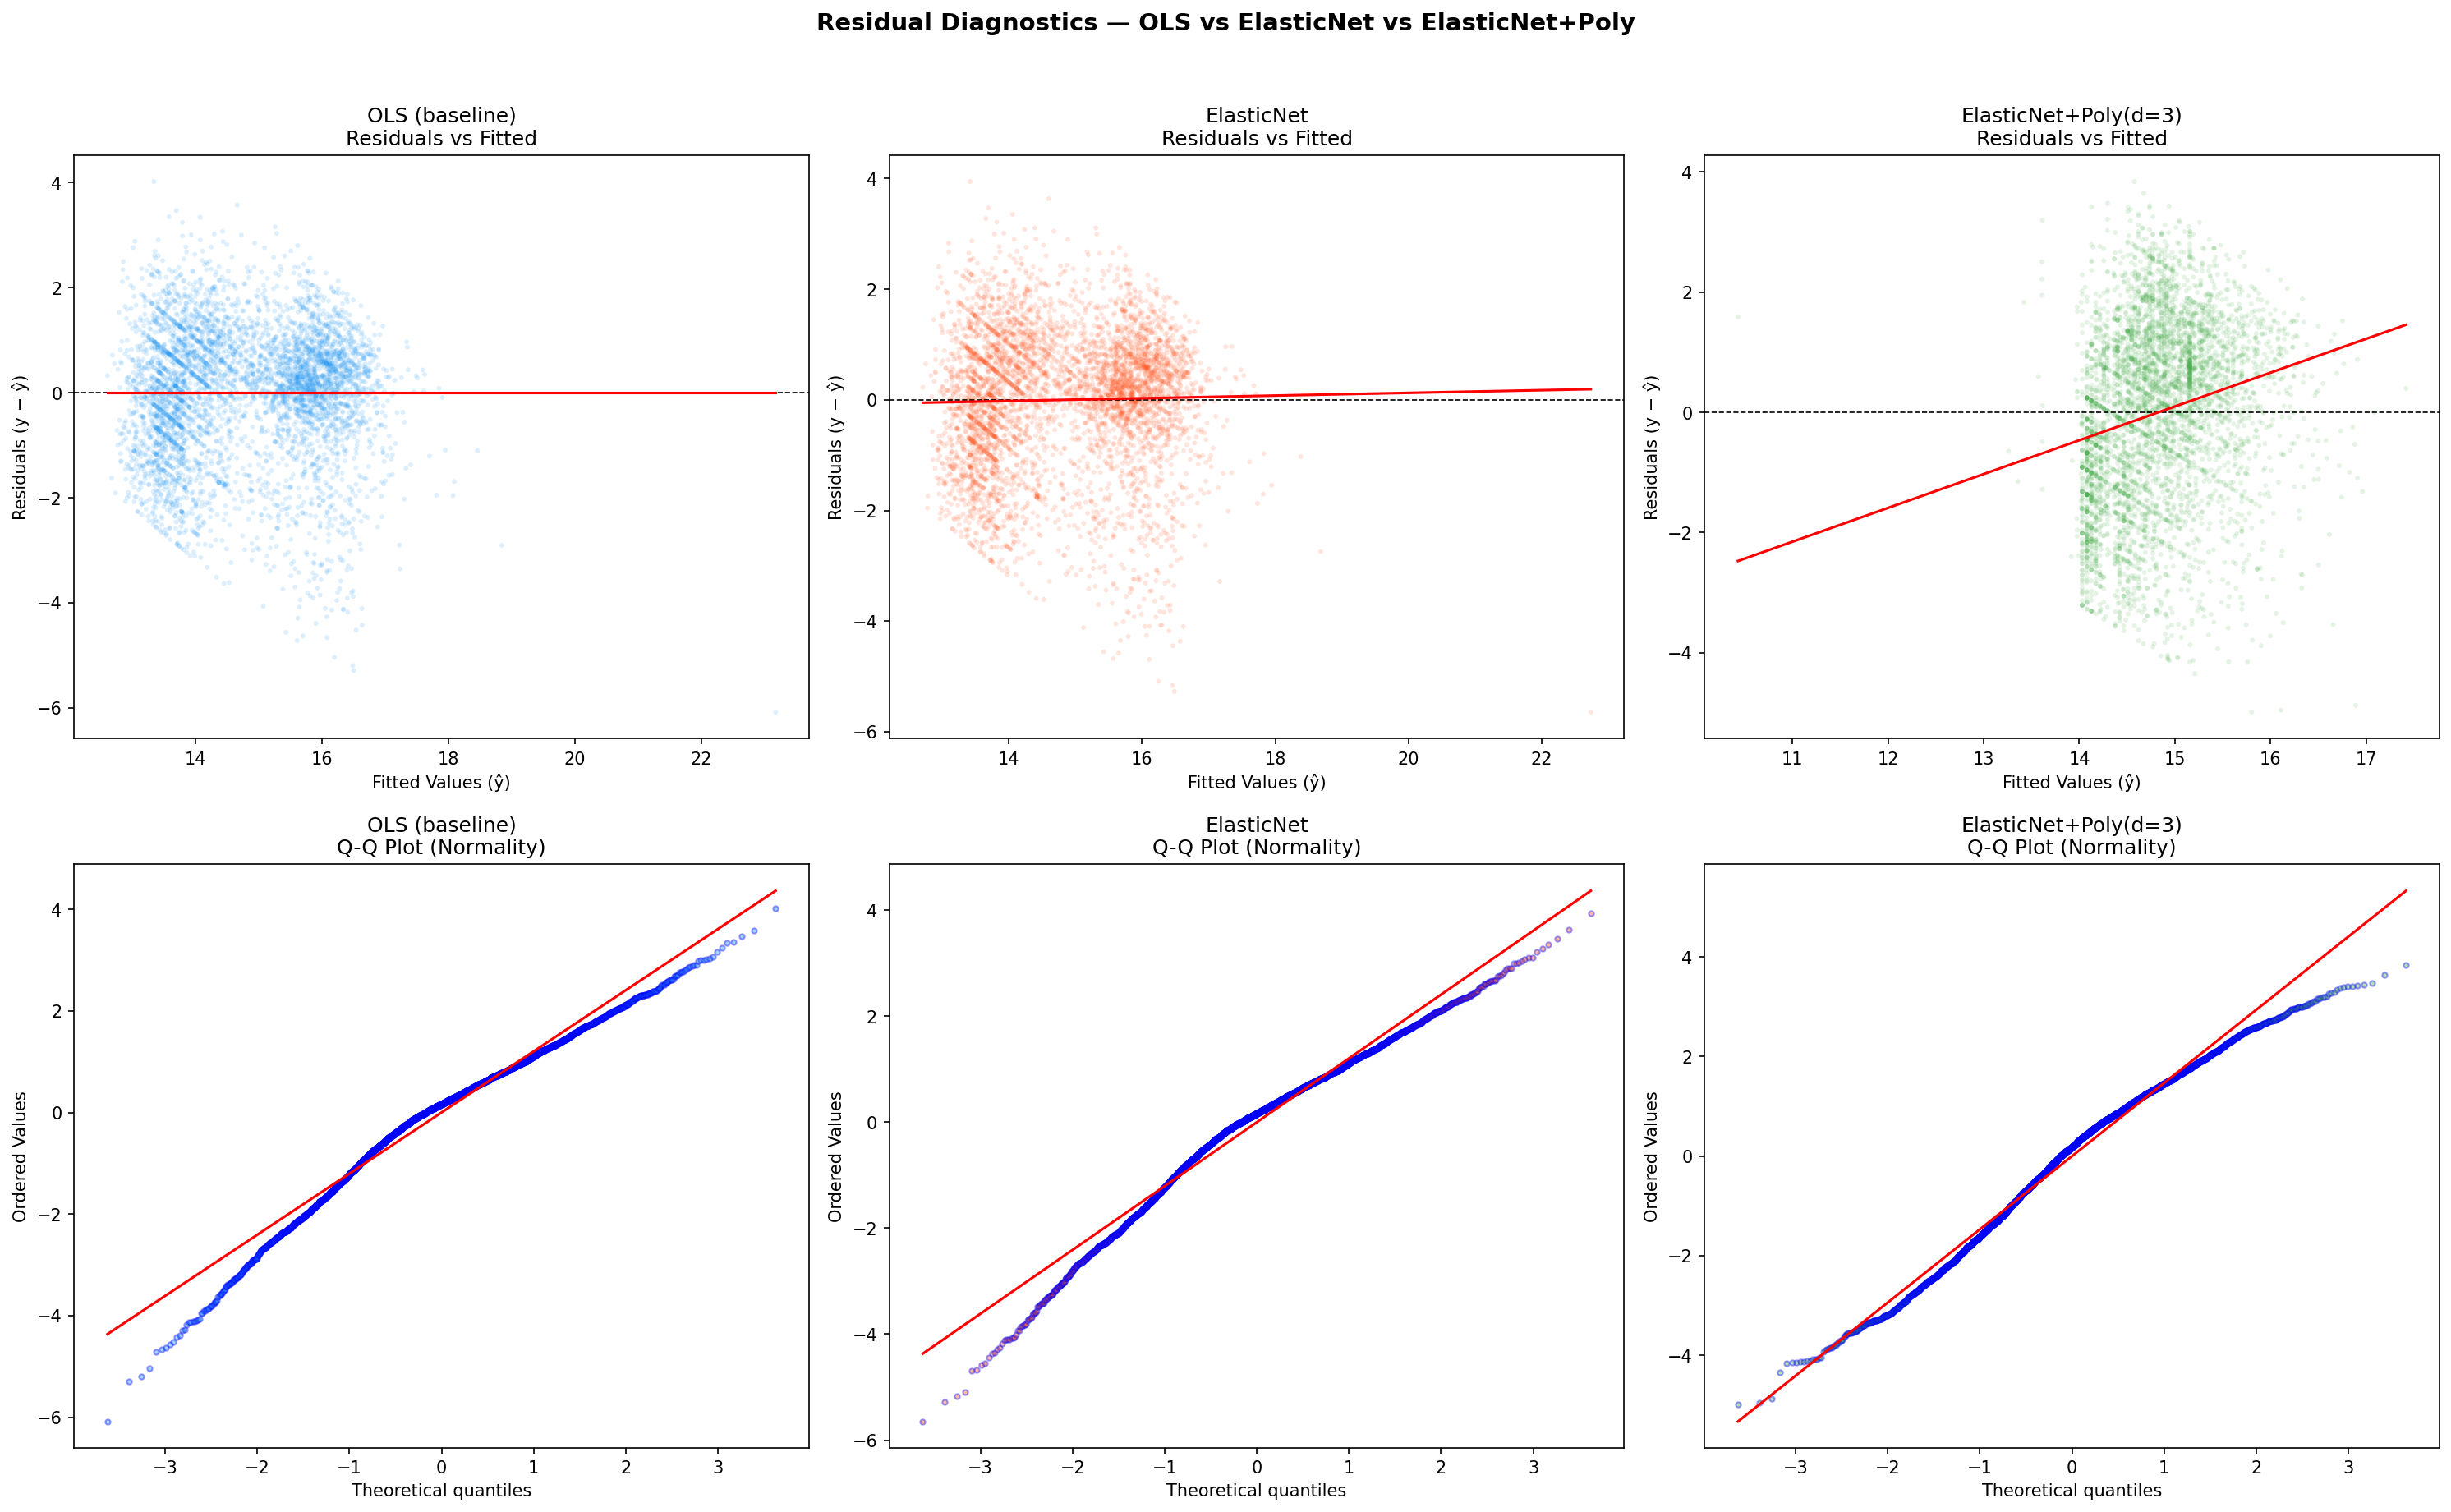
\includegraphics[width=\textwidth]{fig_residual_comparison.png}
    \caption{Chẩn đoán phần dư cho 3 mô hình đại diện. \textbf{Hàng trên:} Residuals vs Fitted Values — kiểm tra tuyến tính và đồng phương sai. Đường đỏ là đường trendline LOWESS; gần nằm ngang ở mức 0 cho thấy giả thiết GM3 được thỏa mãn. \textbf{Hàng dưới:} Normal Q-Q Plot — so sánh phân bố phần dư với chuẩn lý thuyết. Lệch nhẹ ở đuôi là chấp nhận được với $n > 4000$.}
    \label{fig:residual}
\end{figure}

\begin{figure}[H]
    \centering
    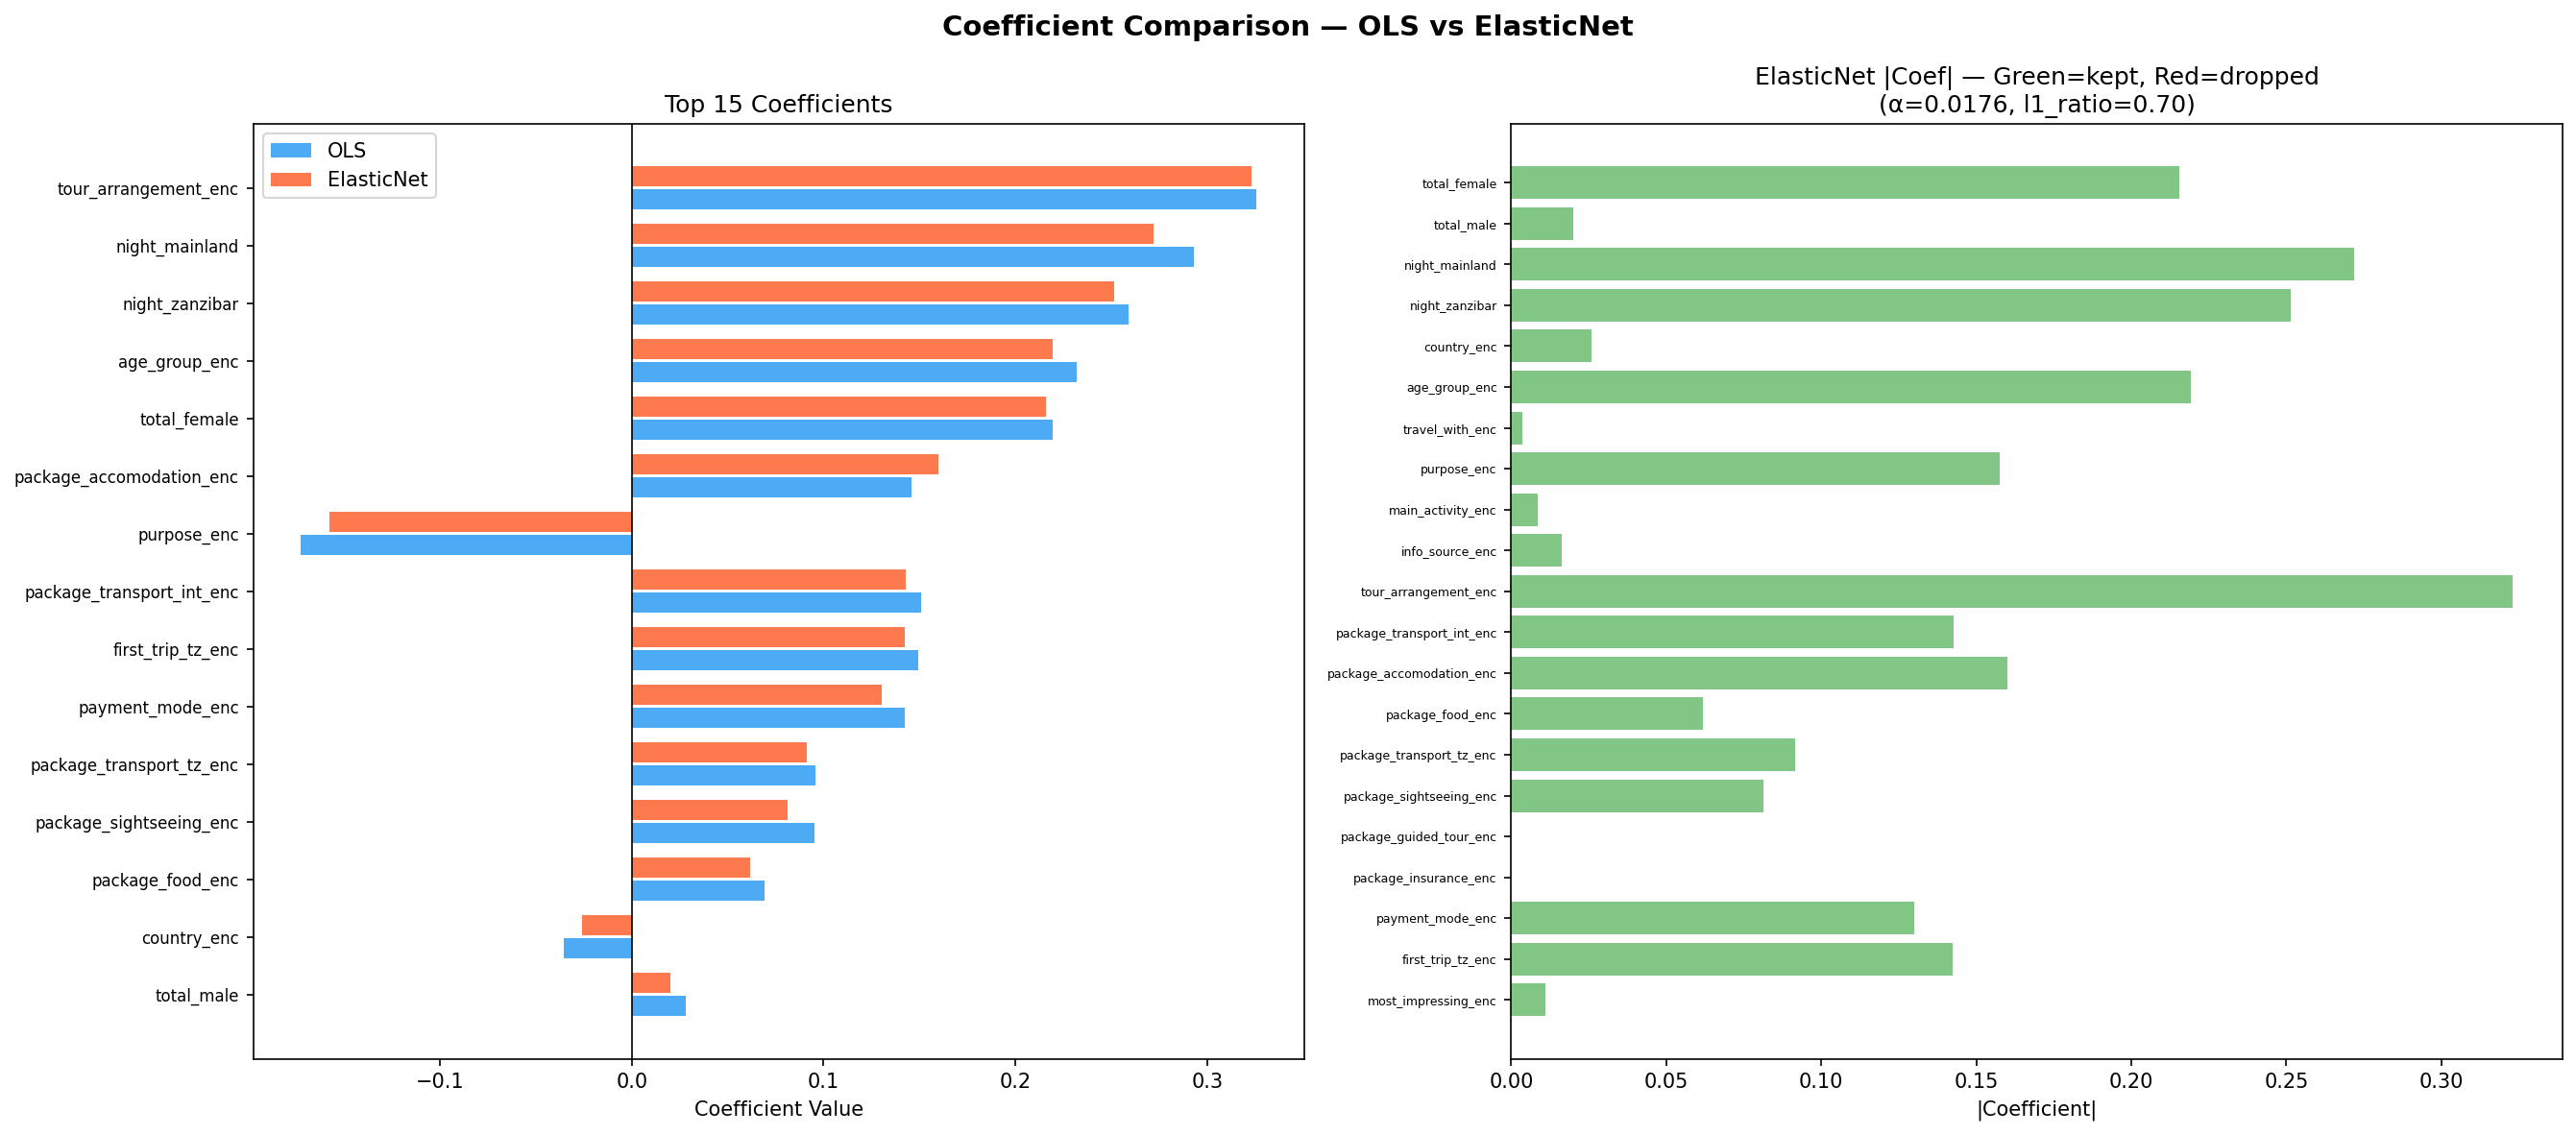
\includegraphics[width=\textwidth]{fig_coefficient_comparison.png}
    \caption{So sánh hệ số OLS vs ElasticNet. \textbf{Trái:} Top 15 đặc trưng theo $|\hat{\beta}|$, hiển thị hiệu ứng shrinkage của ElasticNet (hệ số nhỏ hơn OLS nhưng thứ tự bảo toàn). \textbf{Phải:} Toàn bộ 21 biến với mã màu: xanh = giữ lại ($|\hat{\beta}| > 0$), đỏ = bị loại ($\hat{\beta} = 0$). Hai biến bị loại là \texttt{package\_guided\_tour} và \texttt{package\_insurance}.}
    \label{fig:coef_fig}
\end{figure}

\begin{figure}[H]
    \centering
    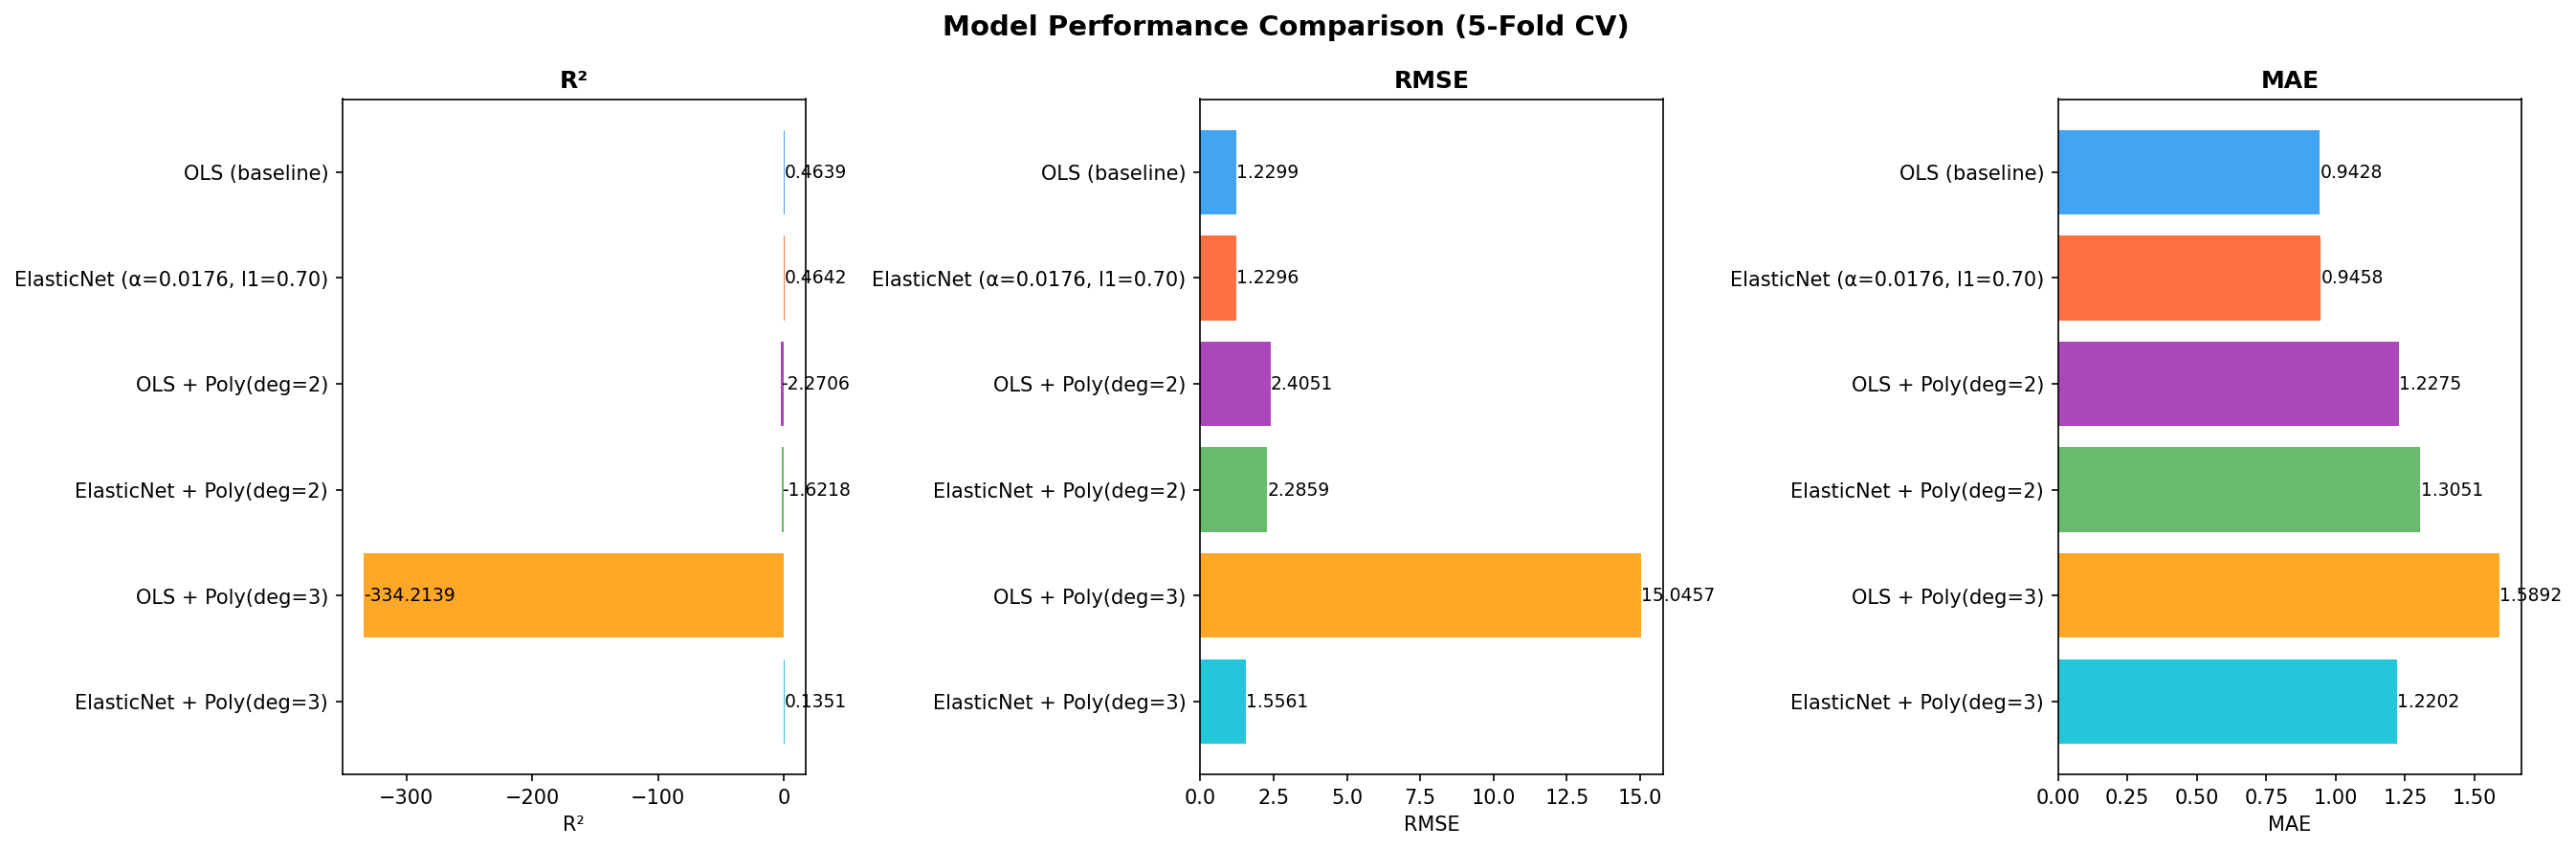
\includegraphics[width=\textwidth]{fig_model_performance.png}
    \caption{So sánh hiệu năng $R^2$, RMSE, MAE của 6 mô hình qua 5-Fold CV. Thanh lỗi biểu thị độ lệch chuẩn qua các fold. OLS và ElasticNet (trên 21 features) vượt trội rõ ràng so với các mô hình Polynomial, cho thấy predictive power chủ yếu đến từ biến categorical.}
    \label{fig:perf}
\end{figure}

% ══════════════════════════════════════════════════════════════
% 5. KẾT LUẬN
% ══════════════════════════════════════════════════════════════
\section{Kết Luận và Đề Xuất}

\subsection{Kết Luận Chính}

Thí nghiệm này cung cấp một cái nhìn toàn diện về ứng dụng Elastic Net và Polynomial Regression vào bài toán dự đoán chi phí du lịch tại Tanzania. Bốn kết luận chính được rút ra:

\begin{enumerate}[leftmargin=1.5em]
    \item \textbf{Elastic Net} ($\alpha = 0.0176$, $\rho = 0.70$) đạt $R^2 = 0.4642$ qua 5-fold CV, vượt trội so với OLS One-Hot ở báo cáo trước ($R^2 = 0.3395$) và nhỉnh hơn OLS baseline mới ($R^2 = 0.4639$). Điểm mạnh không chỉ ở hiệu năng mà còn ở khả năng \textbf{feature selection tự động}: loại bỏ 2/21 biến dư thừa (\texttt{package\_guided\_tour} và \texttt{package\_insurance}), tạo mô hình gọn gàng và diễn giải được hơn.

    \item \textbf{Polynomial Regression} (bậc 2 và 3) trên 4 biến numeric không cải thiện mô hình ($R^2$ giảm mạnh xuống 0.12--0.14). Nguyên nhân cốt lõi là predictive power nằm chủ yếu ở các biến categorical (đặc biệt là \texttt{tour\_arrangement}), và mối quan hệ giữa biến numeric với target không có dạng phi tuyến phức tạp.

    \item \textbf{Feature importance:} Thứ tự quan trọng là \texttt{tour\_arrangement} $>$ \texttt{night\_mainland} $>$ \texttt{night\_zanzibar} $>$ \texttt{age\_group}. Chi phí du lịch phụ thuộc mạnh vào hình thức tổ chức tour (Independent vs Package) và thời gian lưu trú tại các vùng khác nhau.

    \item \textbf{Label Encoding kết hợp log1p target} cho kết quả tốt hơn One-Hot Encoding khi số chiều thấp (21 vs 186 features), một bài học thực tế quan trọng cho các bài toán tương tự có nhiều biến categorical.
\end{enumerate}

\subsection{Đề Xuất Cải Thiện}

Dựa trên phân tích kết quả, nhóm đề xuất các hướng cải thiện theo thứ tự ưu tiên:

\begin{enumerate}[leftmargin=1.5em]
    \item \textbf{Feature Engineering nâng cao:} Tạo interaction terms giữa biến categorical như \texttt{country} $\times$ \texttt{tour\_arrangement} (một số quốc gia có tỷ lệ đặt tour trọn gói cao hơn, điều này có thể có ý nghĩa kinh tế), hoặc \texttt{age\_group} $\times$ \texttt{main\_activity}. Đây sẽ hiệu quả hơn nhiều so với polynomial trên biến numeric.

    \item \textbf{Target Encoding:} Thay Label Encoding bằng Target Encoding hoặc CatBoost Encoding để khai thác thông tin từ biến mục tiêu khi mã hóa categorical, đặc biệt hữu ích cho biến \texttt{country} với 70+ giá trị.

    \item \textbf{Mô hình phi tuyến:} Sử dụng Gradient Boosting (XGBoost, LightGBM) để bắt các mối quan hệ phi tuyến phức tạp và tương tác đa chiều mà hồi quy tuyến tính không thể mô tả. Dựa trên kết quả của nhóm với Ridge ($R^2 \approx 0.35$) và ElasticNet ($R^2 \approx 0.46$), có khả năng cao XGBoost có thể đạt $R^2 > 0.6$ trên cùng bộ dữ liệu.

    \item \textbf{Stratified K-Fold:} Chia fold theo quantile của target để đảm bảo mỗi fold có phân bố target tương tự nhau, tránh trường hợp một fold tình cờ chứa nhiều outliers và làm sai lệch đánh giá.
\end{enumerate}

% ══════════════════════════════════════════════════════════════
% REFERENCES
% ══════════════════════════════════════════════════════════════
\newpage
\begin{thebibliography}{9}

\bibitem{zou2005}
H.~Zou and T.~Hastie, ``Regularization and variable selection via the elastic net,'' \textit{Journal of the Royal Statistical Society: Series B}, vol.~67, no.~2, pp.~301--320, 2005.

\bibitem{tibshirani1996}
R.~Tibshirani, ``Regression shrinkage and selection via the lasso,'' \textit{Journal of the Royal Statistical Society: Series B}, vol.~58, no.~1, pp.~267--288, 1996.

\bibitem{hoerl1970}
A.~E.~Hoerl and R.~W.~Kennard, ``Ridge regression: Biased estimation for nonorthogonal problems,'' \textit{Technometrics}, vol.~12, no.~1, pp.~55--67, 1970.

\bibitem{hastie2009}
T.~Hastie, R.~Tibshirani, and J.~Friedman, \textit{The Elements of Statistical Learning}, 2nd~ed. Springer, 2009.

\bibitem{wooldridge2013}
J.~M.~Wooldridge, \textit{Introductory Econometrics: A Modern Approach}, 5th~ed. South-Western Cengage Learning, 2013.

\end{thebibliography}

\end{document}